\begin{exercise}{Igloo}{3}{Spé}
{Diffusion thermique}{bermu}

Considérons un igloo dans la région polaire reculée du Yukon. C'est une calotte hémisphérique de rayon $R$ et d'épaisseur $h$ de glace. On est au mois de février, le plus rude de l'année, où les nuits sont très froides : peut-on survivre au froid dans l'igloo durant la nuit ?

\begin{questions}
    \questioncours Effectuer un bilan thermique sur un élément de volume de glace de l'igloo et en déduire une équation  de la chaleur. De même, établir l'équation de la chaleur à l'intérieur l'igloo.
    
    \question (\textsf{Cas stationnaire}) Résoudre l'équation dans le cas ou la température est constante, pour une température extérieure $T_0$ dont on choisira une valeur pertinente.
    
    \question (\textsf{Cas harmonique}) Maintenant, on impose un forçage extérieur en $\Delta T e^{i\omega t}$. \\ Justifier cette écriture et donner des ordres de grandeur judicieux pour $\Delta T$ et $\omega$.
    
    \question Réécrire l'équation de diffusion et dégager un paramètre de longueur $H$ pertinent, dont on donnera une interprétation et un ordre de grandeur.
    
    \question (\textsf{Résolution de l'équation}) En introduisant le changement de variable $f(r) = T(r)\times r$, résoudre l'équation.
    
    \question (\textsf{Bilan}) Peut-on survivre à la nuit polaire dans un igloo ?
    
    \question (\textsf{Bonus}) Quid des variations annuelles ?
\end{questions}

\paragraph{Données :}

\begin{center}
    \begin{tabular}{r|ll}
       &  Air      & Glace  \\ \hline
    Capacité thermique volumique (kJ$\cdot$K$^{-1}\cdot$m$^{-3}$) &
    1,3 & 1,9 \\
    Conductivité thermique (W$\cdot$m$^{-1}\cdot$K$^{-1}$) &
    0,02 & 2,1 \\ \hline
    \end{tabular}
\end{center}

Puissance thermique rayonnée par le corps humain $P_\text{h} \sim 100$ W.

\begin{figure}[H]
    \centering
    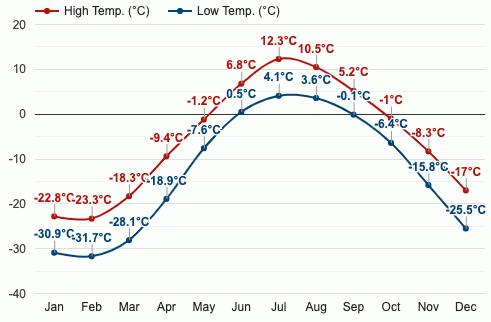
\includegraphics[scale=1.3]{thermo/diffusion/diffusionthermique/igloo.png}
    \caption{Variation de température à Whitehorse, Yukon, Canada.}
\end{figure}

\bigskip

\begin{center}
    \begin{minipage}{15cm}
        \textit{
        "The land itself was a desolation, lifeless, without movement, so lone and cold that the spirit of it was not even that of sadness. There was a hint in it of laughter, but of laughter more terrible than any sadness [...], a laughter cold as the frost and partaking of the grimness of infallibility. It was the Wild, the savage, frozen-hearted Northland Wild."}
        
        --- \quad \emph{White Fang}, Jack London
    \end{minipage}
\end{center}


\end{exercise}

\begin{solution}
\begin{questions}
    \question Voir le cours, on trouve l'équation de la chaleur
    \begin{align*}
        \pdv{T}{t} = \kappa \Delta T
    \end{align*}
    avec $\kappa = \frac{\lambda}{\mu c}$ la diffusivité thermique. Dans la couche de glace, les transferts thermiques se font par conduction. À l'intérieur de l'igloo il y a de l'air, les transferts thermiques se font par convection (bien plus rapidement que par conduction), on peut donc supposer que l'air à l'intérieur de l'igloo à une température homogène $T_i(t)$.
    
    \question (\textsf{Cas stationnaire}) Dans ce cas, on a $T = T(r)$, la température extérieure $T_0$ est constante ainsi que la température intérieure $T_i$. On a donc une équation de Laplace à résoudre : 
    \begin{align*}
        \Delta T = 0
    \end{align*}
    Avec comme condition aux limites :
    \begin{itemize}
        \item À l'extérieur de l'igloo, on prend une condition aux limites de type Dirichlet $T(R) = T_0$ (on pourrait aussi utiliser un modèle de flux conducto-convectif mais cela complexifierait le problème donc inutile de se lancer là-dedans si le sujet/l'examinateur ne vous y invite pas)
        \item À l'extérieur de l'igloo, on a une condition non pas sur la température (on ne connaît pas $T_i$ puisque c'est ce qu'on cherche) mais sur sa dérivée (condition de Neumann). Il faut dire que le flux total de chaleur sortant de l'intérieur de l'igloo $\phi$ est égal à la puissance thermique émise par la personne à l'intérieur $P$\footnote{Ordre de grandeur à connaître : la puissance thermique émise par un être humain lambda est de l'ordre de 100 W.}. Ce flux total est donc $\phi = \frac12 4\pi (R-h)^2 j(R-h) = P$, avec $j(R-h) = -\lambda \pdv{T}{r}(R-h)$.
    \end{itemize}
    On résout l'équation de Laplace (en utilisant la formule du laplacien en sphérique si on la connaît, en la retrouvant en faisant un bilan de chaleur sur une calotte hémisphérique infinitésimale sinon, cf cours) :
    \begin{align*}
         \frac1{r^2} \pdv{r}\qty(r^2\pdv{T}{r}) &= 0 \\
         \pdv{T}{r} &= -\frac{A}{r^2} \\
         T(r) &= B + \frac{A}{r}
    \end{align*}
    Et en utilisant que $T(R) = T_0$ et $\pdv{T}{r}(R-h) = -\frac{P}{2\pi \lambda (R-h)^2}$, on trouve $A = \frac{P}{2\pi \lambda}$ et $B = T_0 - \frac{P}{2\pi \lambda R}$, soit 
    \begin{align*}
        T(r) = T_0 + \frac{P}{2\pi \lambda}\qty(\frac1r-\frac1R)
    \end{align*}
    À ce stade, comme d'habitude, on vérifie que tout est bien homogène, on remarque que $T$ diminue lorsque $r$ augmente ce qui est toujours rassurant, et on peut même faire une petite application numérique pour trouver $T_i = T(R-h)$ en prenant des valeurs raisonnables de $P$, $R$ et $h$, $\lambda_{\text{glace}}$ étant fournie.
    
    \question (\textsf{Cas harmonique}) Cette fois-ci, la température extérieure n'est plus $T0$ mais $T_0 + \Delta T e^{i\omega t}$. Interprétation physique, cela correspond à une variation périodique de la température, le plus naturel a priori étant d'assimiler ceci à la variation des températures du rythme jour / nuit, on prendra donc pour les applications numériques $\omega = \frac{2\pi}{1\text{ jour}}$ et $\Delta T$ peut être obtenu en regardant l'écart moyen entre les deux courbes de la figure fournie.
    
    \question On a déjà déterminé la partie stationnaire de $T$, on étudie maintenant la partie oscillante. Cette fois-ci on doit écrire l'équation de diffusion dans toute sa généralité. Comme toujours dans ce genre de situations, on évite les fastidieux calculs du régime transitoire et on se place en régime permanent, on a donc $T(r, t) = \underline{T}(r) e^{i\omega T}$ avec $\underline{T} \in \mathbb{C}$. L'équation de la diffusion devient donc
    \begin{align*}
        i \omega \underline{T} = \kappa \Delta \underline{T} 
    \end{align*}
    Qui est donc une équation de Poisson
    \begin{align*}
        \Delta \underline{T} = i \frac{\underline{T}}{H^2}
    \end{align*}
    avec $H = \sqrt{\frac{\kappa}{\omega}}$ la taille caractéristique du problème. Puisque $\kappa$ la diffusivité thermique est une constante de diffusion comme son nom l'indique, $H$ est bien homogène à une longueur. Ouf !
    
    \question (\textsf{Résolution de l'équation}) Comme avant on écrit l'équation de Poisson :
    \begin{align*}
        \frac1{r^2} \pdv{r}\qty(r^2\pdv{T}{r}) &= i \frac{\underline{T}}{H^2}
    \end{align*}
    Qui a priori n'est pas triviale à résoudre. Malheur ! Heureusement, on peut faire confiance au colleur, qui nous a généreusement fourni un astucieux changement de variable (merci à lui). Suivant ses instruction les yeux fermés, on pose $f(r) = r \underline{T}(r)$ et on exprime l'équation en fonction de $f$ :
    \begin{align*}
        \pdv{r}\qty(r^2\pdv{r}\qty(\frac{f}{r})) &= i r\frac{f}{H^2} \\
        \pdv{r}\qty(r\pdv{f}{r} - f) &= i r\frac{f}{H^2} \\
        \pdv{f}{r} + r\pdv[2]{f}{r} - \pdv{f}{r} &= i r\frac{f}{H^2} \\
        \pdv[2]{f}{r} &= i \frac{f}{H^2}
    \end{align*}
    Qui est une équation d'oscillateur harmonique dont on connaît les solutions. Youpi ! \\
    Puisque $i = \qty(e^{i\frac{\pi}{4}})^2 = \qty(\frac{1+i}{\sqrt{2}})^2$, on peut réécrire l'équation
    \begin{align*}
        \pdv[2]{f}{r} &= \qty(\frac{1+i}{\sqrt{2}H})^2 f
    \end{align*}
    Dont les solutions sont évidentes : $f(r) = A\exp(\frac{1+i}{\sqrt{2}H}r) + B\exp(-\frac{1+i}{\sqrt{2}H}r)$, d'où l'on déduit $\underline{T}(r)$.
    
    \question (\textsf{Bilan}) La détermination exacte de $\underline{T}(r)$ ici est fastidieuse (il faudrait utiliser une forme astucieusement choisie de $f$ et appliquer rigoureusement les conditions aux limites en partie réelle et imaginaire). L'important est de voir que le module de la température varie proportionnellement à $e^{\frac{r}{H}}$, on peut donc dire grossièrement que l'igloo est ou pas sensible aux variations journalières de température selon que $h$ est plus grand ou plus petit que $H$. Une application numérique et un commentaure sont ici bienvenus.
    
    \question (\textsf{Bonus}) Il suffit comme précédemment d'utiliser la linéarité de l'équation pour superposer une seconde variation périodique de température $\Delta T '$ (pouvant être lu sur le graphe fourni) de fréquence $\omega' = \frac{2\pi}{1 \text{an}}$, et de reprendre le résultat précédent avec la nouvelle valeur $H'$.
\end{questions}

Pour conclure, un exercice qui commence par une question de cours standard (démonstration de l'équation de la chaleur) et se poursuit par une application très classique (résolution d'une équation de Laplace unidimensionnelle en géométrie sphérique). La situation est ensuite complexifiée par l'ajout d'une variation périodique, il suffit alors de suivre les raisonnements habituels en se laissant guider par les questions. Certaines questions sont volontairement imprécises, comme très souvent dans les exercices d'oraux, afin d'encourager la prise d'initiative et la discussion.

Il est de plus agrémenté d'un joli texte de Jack London, ce qui n'est pas sans contribuer à son intérêt !

\end{solution}